% -*- compile-command: "make slides.pdf" -*-
\documentclass{beamer} 
\usepackage{tikz}
\usepackage{amsmath,amssymb}
\usepackage{hyperref}
\usepackage{graphicx}

\usepackage[utf8]{inputenc}%for french accents. 
%\usepackage{appendixnumberbeamer}

\addtobeamertemplate{navigation symbols}{}{%
    \usebeamerfont{footline}%
    \usebeamercolor[fg]{footline}%
    \hspace{1em}%
    \insertframenumber/\inserttotalframenumber
}

\DeclareMathOperator*{\argmin}{arg\,min}
\DeclareMathOperator*{\Lik}{Lik}
\DeclareMathOperator*{\Peaks}{Peaks}
\DeclareMathOperator*{\Segments}{Segments}
\DeclareMathOperator*{\argmax}{arg\,max}
\DeclareMathOperator*{\maximize}{maximize}
\DeclareMathOperator*{\minimize}{minimize}
\newcommand{\sign}{\operatorname{sign}}
\newcommand{\RR}{\mathbb R}
\newcommand{\ZZ}{\mathbb Z}
\newcommand{\NN}{\mathbb N}
\definecolor{pDPA}{HTML}{1B9E77}
\definecolor{PELT}{HTML}{D95F02}
\definecolor{FPOP}{HTML}{7570B3}
\newcommand{\algo}[1]{\textcolor{#1}{#1}}
\definecolor{PDPA}{HTML}{66C2A5}
\definecolor{CDPA}{HTML}{FC8D62}
\definecolor{GPDPA}{HTML}{4D4D4D}




% Set transparency of non-highlighted sections in the table of
% contents slide.
\setbeamertemplate{section in toc shaded}[default][100]
\AtBeginSection[]
{
  \setbeamercolor{section in toc}{fg=red} 
  \setbeamercolor{section in toc shaded}{fg=black} 
  \begin{frame}
    \tableofcontents[currentsection]
  \end{frame}
}

\begin{document}

\title{Same vs. other cross-validation in supervsied machine learning}
\author{
  Toby Dylan Hocking\\
  toby.hocking@nau.edu
}

\maketitle

\section{Introduction to machine learning}

\begin{frame}
  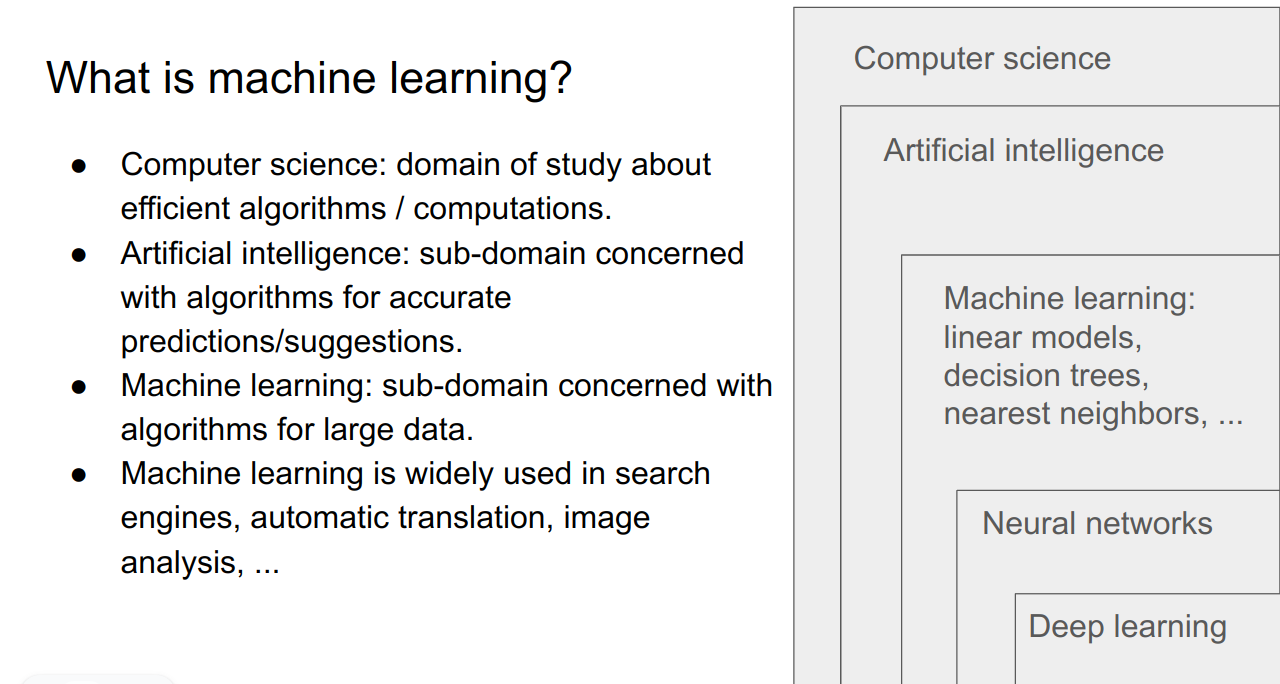
\includegraphics[width=\textwidth]{figure-ai-vs-ml}
\end{frame}

\begin{frame}
  \frametitle{Machine learning intro: image classification example}
  ML is all about learning predictive functions $f(x)\approx y$, where 
  \begin{itemize}
  \item Inputs/features $x$ can be easily computed using traditional
    algorithms, e.g. matrix of pixel intensities in an image.
  \item Outputs/labels $y$ are what we want to predict, easy to get by
    asking a human, but hard to compute using traditional algorithms,
    e.g. image class.
  \item Input $x$ = image of digit, output $y\in\{0,1,\dots,9\}$, \\--
    this is a classification problem with 10 classes.\\
  $f(
\includegraphics[height=1cm]{mnist-0})=0$,
  $f(
\includegraphics[height=1cm]{mnist-1})=1$
\item Traditional/unsupervised algorithm: I give you a pixel intensity matrix
  $x\in\RR^{16\times 16}$, you code a function $f$ that returns one of
  the 10 possible digits. Q: how to do that?
  \end{itemize}
\end{frame}

\begin{frame}
  \frametitle{Supervised machine learning algorithms}

  I give you a training data set with paired inputs/outputs, e.g.

  \begin{center}
    \Huge $y=$\ 0 1 2 3 4 5 6 7 8 9

$X=$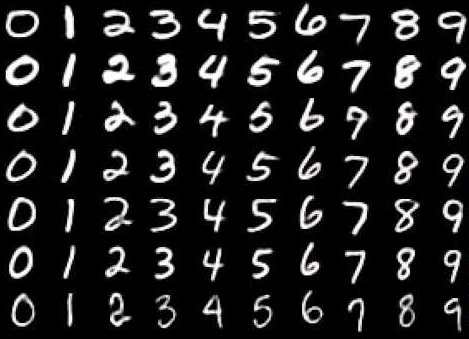
\includegraphics[height=1.9in]{mnist-digits}
  \end{center}

  Your job is to code an algorithm that learns the function $f$ from
  the training data. (you don't code $f$)
  
  \scriptsize Source: github.com/cazala/mnist
\end{frame}

\begin{frame}
  \frametitle{Supervised machine learning algorithms}

  \textbf{Can} be used whenever a knowledgeable/skilled
  human can easily/quickly/consistently create a large database of
  labels for training.

  \vskip 1cm

  \textbf{Should} be used if it is not easy to code the function $f$
  for predicting the labels (using traditional/unsupervised
  techniques).

  \vskip 1cm

  \textbf{Accurate} if the test data, on which you want to use $f$, is
  similar to the train data (input to learning algorithm).

\end{frame}



\begin{frame}
  \frametitle{Advantages of supervised machine learning}

  \begin{center}
      \begin{tabular}{cc}
        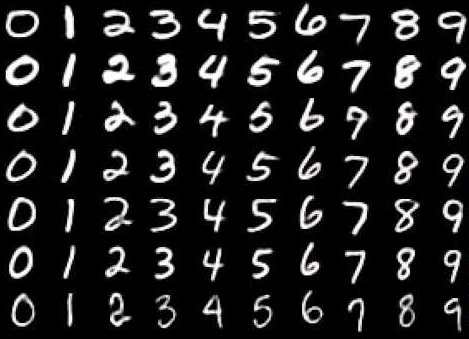
\includegraphics[height=1.5in]{mnist-digits} &
  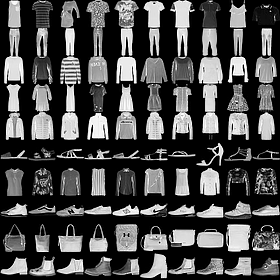
\includegraphics[height=1.5in]{fashion-mnist-sprite-some}  
  \end{tabular}
  \end{center}
  \vskip -0.2cm
  
  \begin{itemize}
  \item Input $x\in\RR^{16\times 16}$, output $y\in\{0,1,\dots,9\}$ types the same!
  \item Can use same learning algorithm regardless of pattern.
  \item Pattern encoded in the labels (not the algorithm).
  \item Useful if there are many un-labeled data, but few labeled data
    (or getting labels is long/costly).
  \item State-of-the-art accuracy (if there is enough training data).
  \end{itemize}

  \scriptsize Sources: github.com/cazala/mnist, github.com/zalandoresearch/fashion-mnist

\end{frame}


\begin{frame}
  \frametitle{Learning two different functions using two data sets} Figure from chapter by Hocking TD,
  \textit{Introduction to machine learning and neural networks} for
  book \textit{Land Carbon Cycle Modeling: Matrix Approach, Data
    Assimilation, and Ecological Forecasting} edited by Luo Y (Taylor
  and Francis, 2022).
  \begin{center}
  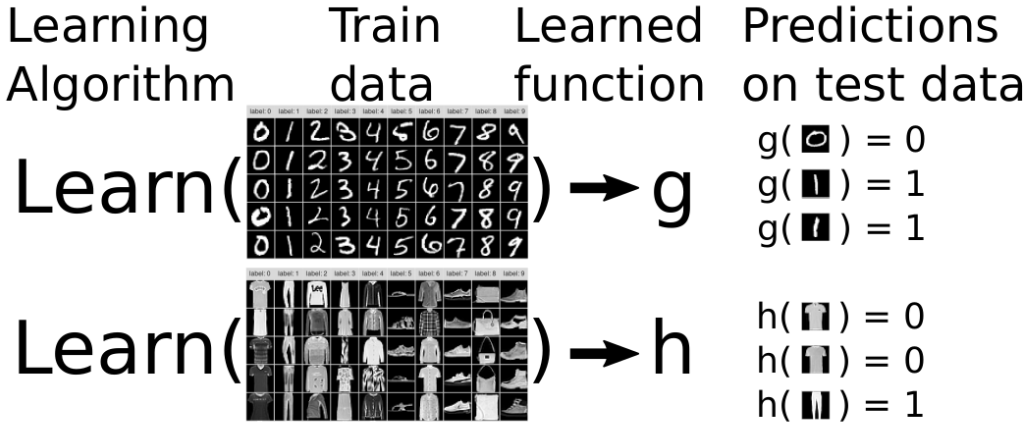
\includegraphics[width=\textwidth]{figure-learn-digits-clothing}
\end{center}
  \textbf{Learn} is a learning algorithm, which outputs
  $g$ and $h$.

  Q: what happens if you do
    $g(
\includegraphics[height=1cm]{fashion-mnist-boot})$, or
    $h(
\includegraphics[height=1cm]{mnist-0})$?
\end{frame}

\begin{frame}
  \frametitle{Learning two different functions using two data sets} 
  \begin{itemize}
  \item What if you do
    $g(
\includegraphics[height=1cm]{fashion-mnist-boot})$, or
    $h(
\includegraphics[height=1cm]{mnist-0})$?
  \item This is a question about \textbf{generalization}: how accurate is the
    learned function on a new/test data set?
  \item ``Very accurate'' if test data are similar enough to train data (best case is i.i.d. = independent and identically distributed)
  \item Predicting childhood autism (Lindly \emph{et al.}), train on
    one year of surveys, test on another.
  \item Predicting carbon emissions (Aslam \emph{et al.}), train on
    one city, test on another.
  \item Predicting presence of trees/fires in satellite imagery
    (Shenkin \emph{et al.}, \emph{Thibaut} \emph{et al.}), train on
    one geographic area/image, test on another.
  \item Predicting fish spawning habitat in sonar imagery (Bodine
    \emph{et al.}), train on one river, test on another.
  \item But how do we check if ``very accurate'' in these situations?
  \end{itemize}
\end{frame}

\section{Proposed same vs. other cross-validation}

\begin{frame}
  \frametitle{$K$-fold cross-validation: a standard algorithm used to estimate the prediction accuracy in machine learning}

  \begin{itemize}
  \item $K=3$ folds shown in figure below, meaning three different
    models trained, and three different prediction/test accuracy rates
    computed.
  \item It is important to use several train/test splits, so we can
    see if there are statistically significant differences between
    algorithms.
  \end{itemize}

  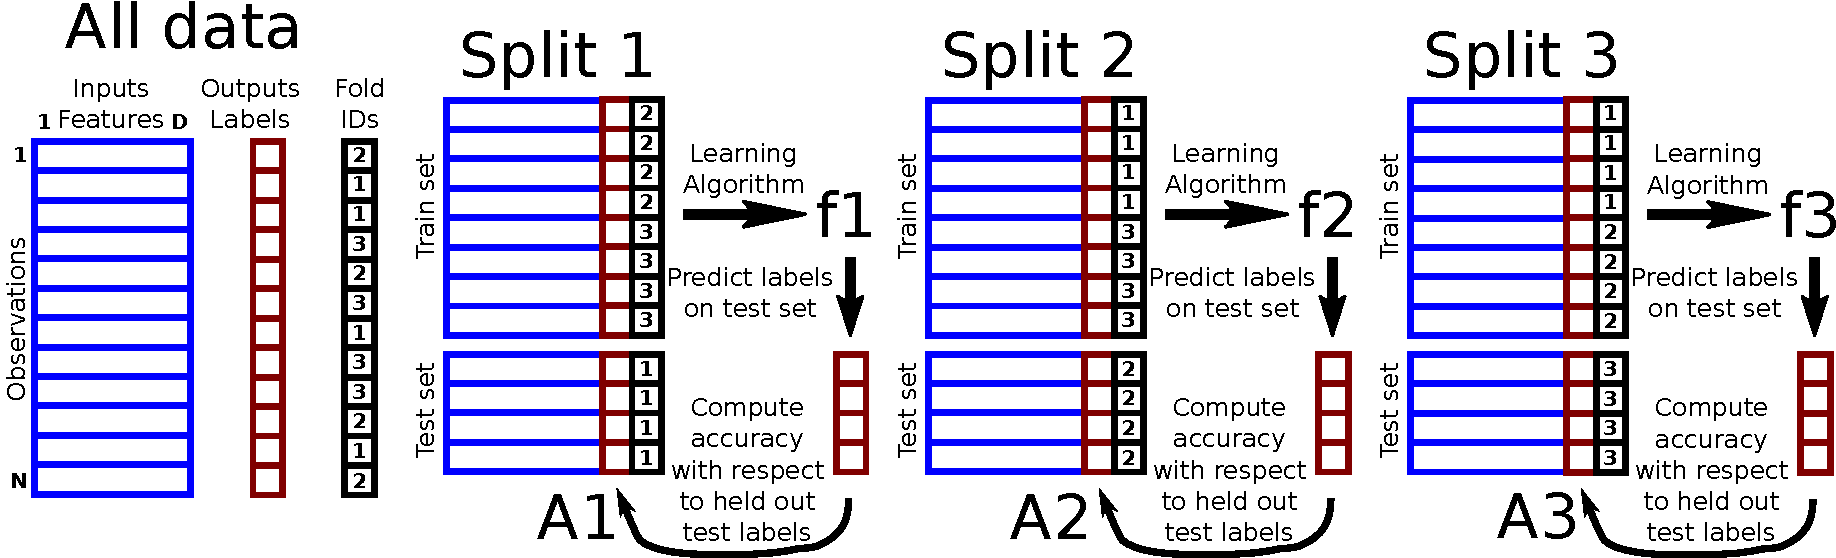
\includegraphics[width=\textwidth]{drawing-cross-validation.pdf}

  \small Hocking TD \emph{Intro. to machine learning and neural
    networks} (2022).
\end{frame}

\begin{frame}
  \frametitle{Example data set: predicting childhood autism}

  \begin{itemize}
  \item Downloaded National Survey of Children's Health (NSCH) data,
    years 2019 and 2020, from
    \url{http://www2.census.gov/programs-surveys/nsch}
  \item One row per person, one column per survey question.
  \item Pre-processing to obtain common columns over the two years,
    remove missing values, one-hot/dummy variable encoding.
  \item Result is $N=46,010$ rows and $D=366$ columns.
  \item 18,202 rows for 2019; 27,808 rows for 2020.
  \item One column is diagnosis with Autism (binary
    classification, yes or no), can we predict it using the others?
  \item Can we combine data from different years?
  \item Can we train on one year, and accurately predict on another?
  \end{itemize}

\end{frame} 


\begin{frame}
  \frametitle{Proposed Same Other Cross-Validation}
  \begin{itemize}
  \item Example: childhood autism prediction data set.
  \end{itemize}
  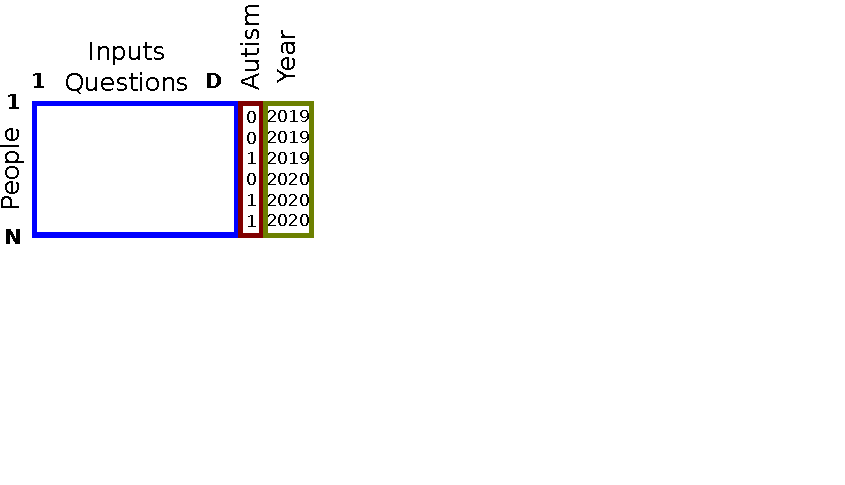
\includegraphics[width=\textwidth]{drawing-cv-same-other-years-1.pdf}
\end{frame}

\begin{frame}
  \frametitle{Proposed Same Other Cross-Validation}
  \begin{itemize}
  \item Train group same as test (=regular $K$-fold CV on 2020).
  \end{itemize}
  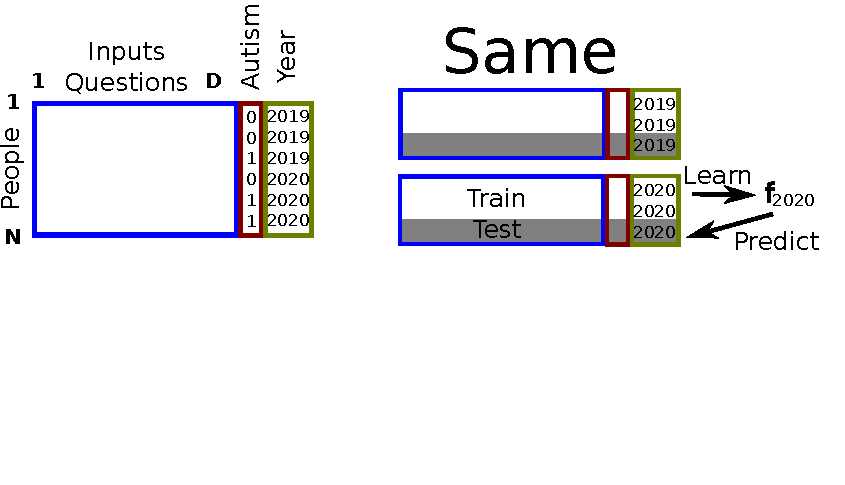
\includegraphics[width=\textwidth]{drawing-cv-same-other-years-2.pdf}
\end{frame}

\begin{frame}
  \frametitle{Proposed Same Other Cross-Validation}
  \begin{itemize}
  \item Train group (2019) different from test (2020).
  \end{itemize}
  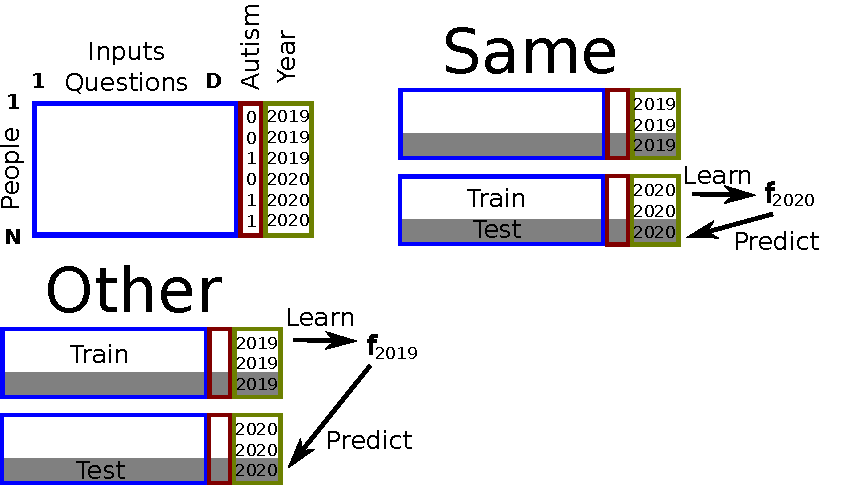
\includegraphics[width=\textwidth]{drawing-cv-same-other-years-3.pdf}
\end{frame}

\begin{frame}
  \frametitle{Proposed Same Other Cross-Validation}
  \begin{itemize}
  \item Repeat for each of $K$ folds, and each test group (2019,2020).
  \end{itemize}
  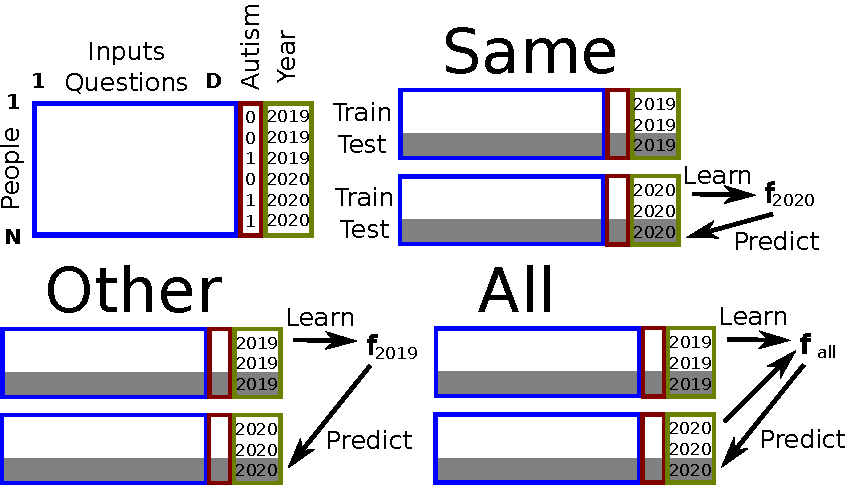
\includegraphics[width=\textwidth]{drawing-cv-same-other-years-4.pdf}
\end{frame}

\begin{frame}
  \frametitle{Proposed Same Other Cross-Validation}
  For a fixed test set from one group:
  
  If train/test are similar/iid,
  \begin{description}
  \item[All] should be most accurate.
  \item[Same/Other] should be less accurate, because there is less
    data available (if other is larger than same, then other should be
    more accurate than same, etc).
  \end{description}

  If train/test are different (not iid),
  \begin{description}
  \item[Same] should be most accurate.
  \item[Other] should be substantially less accurate.
  \item[All] accuracy should be between same and other.
  \end{description}
\end{frame}

\section{Results on real data sets}

\begin{frame}
  \frametitle{Learning algorithms we consider}
  We used the following learning algorithms:
\begin{description}
\item[cv\_glmnet] L1-regularized linear model (feature
  selection). Friedman, \emph{et al.} (2010).
  % Friedman J, Tibshirani R, Hastie T (2010). “Regularization Paths for
  % Generalized Linear Models via Coordinate Descent.” _Journal of
  % Statistical Software_, *33*(1), 1-22. doi:10.18637/jss.v033.i01
  % <https://doi.org/10.18637/jss.v033.i01>.
\item[xgboost] Extreme gradient boosting (non-linear). Chen and Guestrin (2016). 
\item[rpart] Recursive partitioning, decision tree (non-linear, feature selection). Therneau and Atkinson (2023).
  % Therneau T, Atkinson B (2023). _rpart: Recursive Partitioning and
  % Regression Trees_. R package version 4.1.23,
  % <https://CRAN.R-project.org/package=rpart>.
\item[nearest\_neighbors] classic non-linear algorithm, as implemented
  in kknn R package. Schliep and Hechenbichler (2016).
  % Schliep K, Hechenbichler K (2016). _kknn: Weighted k-Nearest
  % Neighbors_. R package version 1.3.1,
  % <https://CRAN.R-project.org/package=kknn>.
\item[featureless] un-informed baseline, ignores all inputs/features,
  and always predicts the most frequent label in train data. For
  example, Autism=No. Nomenclature from mlr3 R package,
  Lang, \emph{et al.}, (2019).
  % Lang M, Binder M, Richter J, Schratz P, Pfisterer F, Coors S, Au Q,
  % Casalicchio G, Kotthoff L, Bischl B (2019). “mlr3: A modern
  % object-oriented machine learning framework in R.” _Journal of Open
  % Source Software_. doi:10.21105/joss.01903
  % <https://doi.org/10.21105/joss.01903>,
  % <https://joss.theoj.org/papers/10.21105/joss.01903>.
\end{description}
Each learning algorithm has different properties (non-linear, feature
selection, etc). For details see Hastie, {\it et al.} (2009) textbook.
\end{frame}

\begin{frame}
  \frametitle{$K$-fold CV on NSCH data (predict autism), year 2020}
  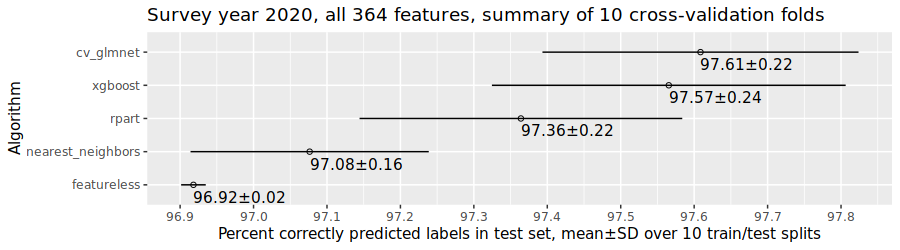
\includegraphics[width=\textwidth]{download-nsch-mlr3batchmark-registry-one-set-all-features-stats.png}

Learning algorithms we consider:
\begin{description}
\item[cv\_glmnet] L1-regularized linear model (feature selection).
\item[xgboost] Extreme gradient boosting (non-linear).
\item[rpart] Recursive partitioning, decision tree (non-linear, feature selection).
\item[nearest\_neighbors] classic non-linear algorithm.
\item[featureless] un-informed baseline, ignores all inputs/features,
  and always predicts the most frequent label in train data (Autism=No
  in this case).
\end{description}

\end{frame}

\begin{frame}
  \frametitle{Same Other for Autism data}
  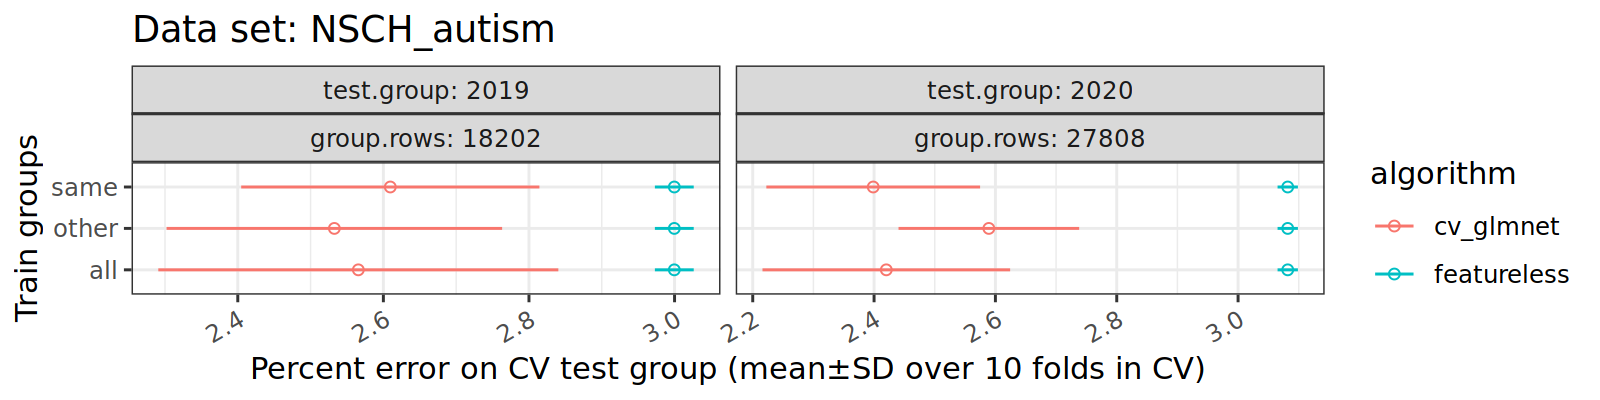
\includegraphics[width=\textwidth]{NSCH_autism_error_glmnet_featureless_mean_SD.png}
  
\end{frame}

\begin{frame}
  \frametitle{Same Other for Autism data}
  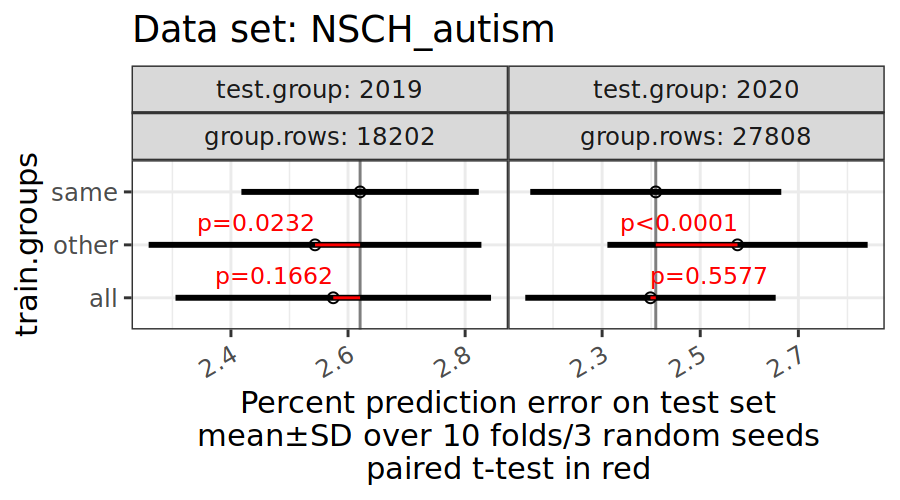
\includegraphics[width=\textwidth]{NSCH_autism_error_glmnet_sizes_mean_SD_pvalue.png}
\end{frame}

\begin{frame}
  \frametitle{Same Other for Autism data}
  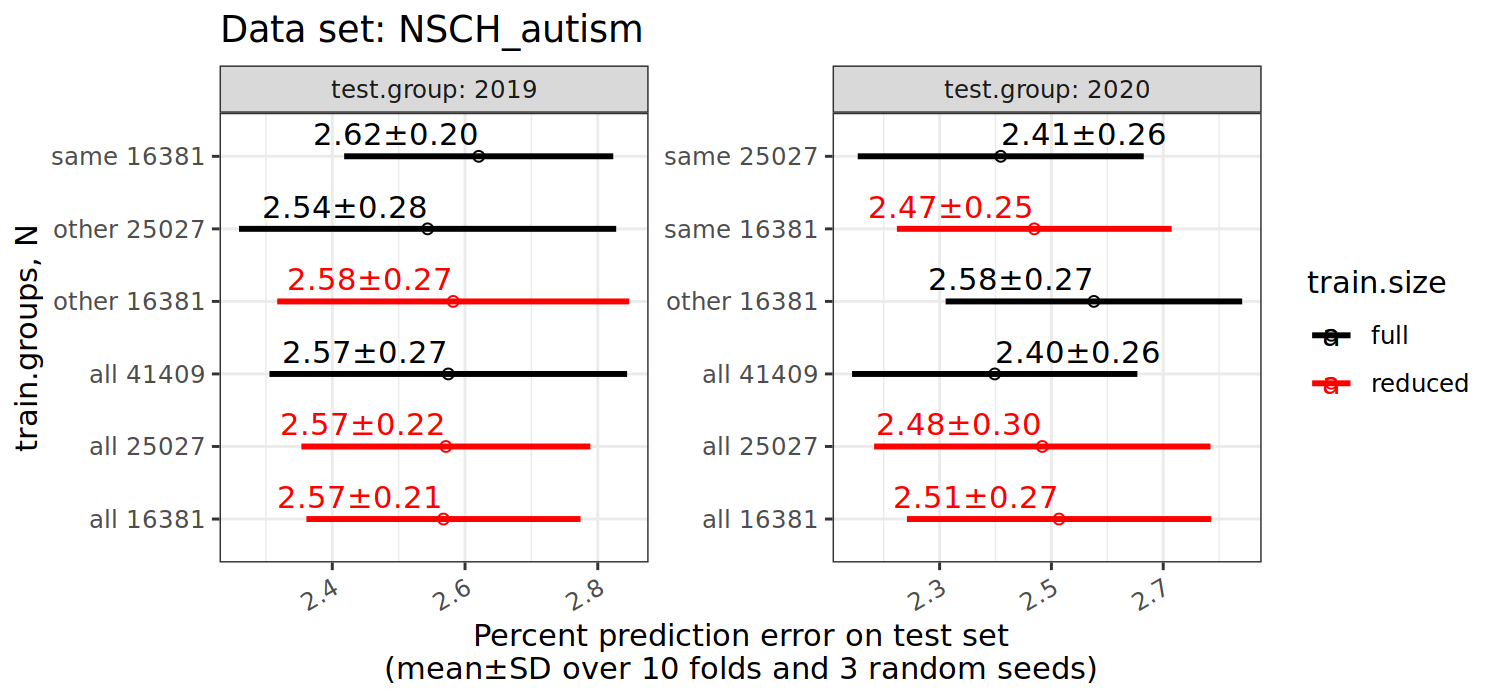
\includegraphics[width=\textwidth]{NSCH_autism_error_glmnet_sizes_mean_sd_more.png}
\end{frame}


\begin{frame}
  \frametitle{Proposed Same Other Cross-Validation}
%  \includegraphics[width=\textwidth]{download-nsch-mlr3batchmark-registry-predict-new-year.png}
  \begin{itemize}
  \item 18,202 rows in 2019, whereas 27,808 in 2020.
  \item For predicting in 2019 (left), training on only 2019 (same) is
    slightly less accurate than training on only 2020 (other), and
    2019+2020 (all). This suggests 2020 data are consistent with the
    pattern in 2019, which is too complex to learn from the limited
    2019 data alone (there is a slight advantage to combining years
    when training).
  \item For predicting in 2020 (right), training on 2019 (other) is slightly less accurate than training on 2020 (same), and 2019+2020 (all). This again suggests that 2019/2020 data are consistent, but there are not enough data in 2019 alone.
  \end{itemize}
% > out.dt[, table(survey_year)]
% survey_year
%  2019  2020 
% 18202 27808 
\end{frame}

\section{Discussion and Conclusions}

\begin{frame}
  \frametitle{Discussion and Conclusions}
  \begin{itemize}
  \item Proposed Same Other Cross-Validation can be used to see if it
    is beneficial to learn using data from different groups (train on
    one group, test/predict on another).
  \item Free/open-source software available: mlr3resampling R package
    on \url{https://github.com/tdhock/mlr3resampling}.
  \item These slides are reproducible, using the code in \url{https://github.com/tdhock/cv-same-other-paper}
  \item Contact: toby.hocking@nau.edu,
    toby.hocking@r-project.org
  \end{itemize}
\end{frame}

\end{document}